\documentclass[border=10pt]{standalone}

\usepackage{tikz}
\usepackage{tikzsymbols}
\usetikzlibrary{calc,patterns,shapes.geometric}

\def\centerarc[#1](#2)(#3:#4:#5){\draw[#1] ($(#2)+({#5*cos(#3)},{#5*sin(#3)})$) arc (#3:#4:#5);}

\begin{document}
	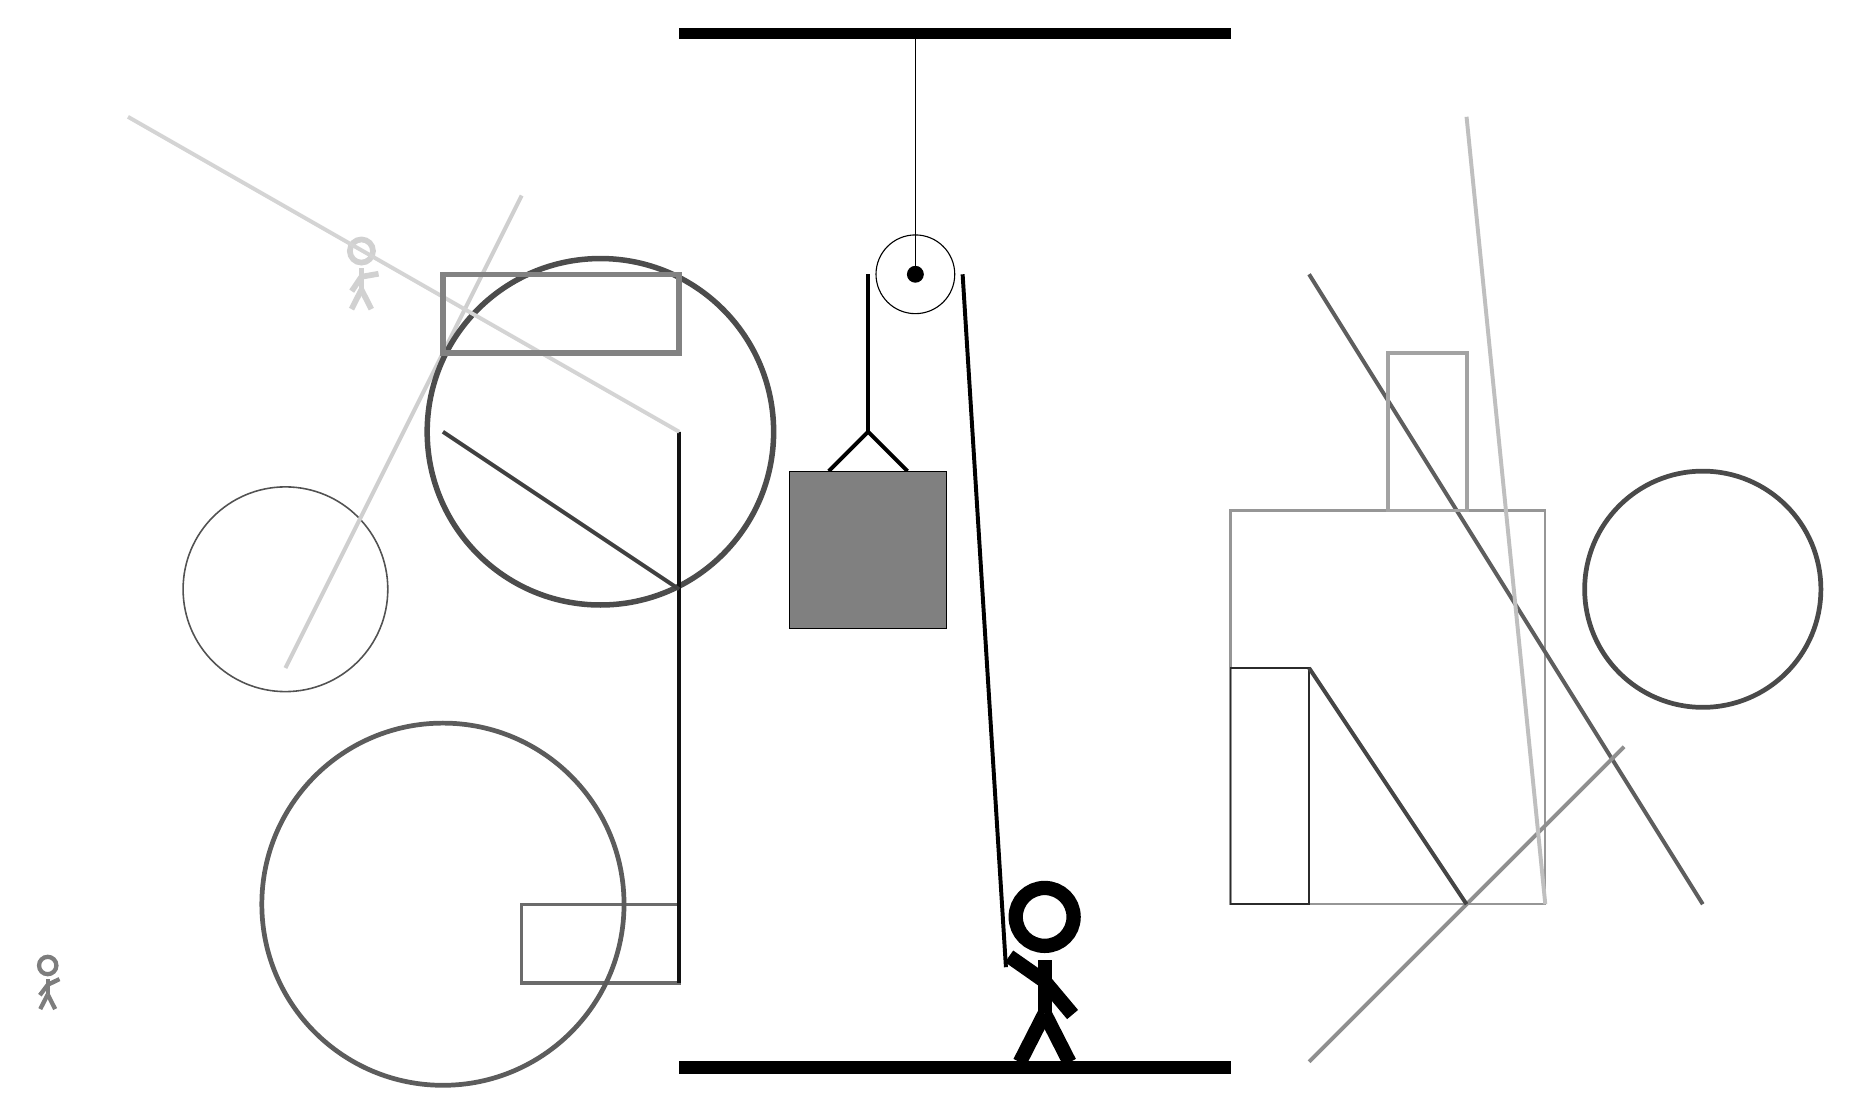
\begin{tikzpicture}
		%%%%% START %%%%%
		
		\draw[fill=black] (-2, 10) rectangle (5, 10.125);
		
		\draw (1, 7) circle (0.5);
		\draw[fill=black] (1, 7) circle (0.1);
		\draw (1, 10) -- (1, 7);
		
		\draw[line width=0.5mm] (-0.1, 4.5) -- (0.4, 5.0) -- (0.9, 4.5);
		\draw[fill=black!50] (-0.6, 4.5) rectangle (1.4, 2.5);
		
		\draw [line width=0.3mm, color=black!41](-7, 2) circle (0.0);
		
		\draw[line width=0.3mm, color=black!41] (5, -1) rectangle (9, 4);
		\draw[line width=0.4mm, color=black!58] (-2, -2) rectangle (-4, -1);
		\draw[line width=0.5mm, color=black!58](7, -3) -- (7, -3);
		
		\draw [line width=0.6mm, color=black!71](11, 3) circle (1.5);
		\draw [line width=0.2mm, color=black!68](-7, 3) circle (1.3);
		\draw[line width=0.5mm, color=black!63](6, 7) -- (11, -1);
		
		\draw[line width=0.5mm, color=black!44](6, -3) -- (10, 1);
		\draw[line width=0.5mm, color=black!19](-4, 8) -- (-7, 2);
		\draw [line width=0.7mm, color=black!70](-3, 5) circle (2.2);
		
		\draw[line width=0.5mm, color=black!93] (-2, -2) rectangle (-2, 5);
		\draw[line width=0.2mm, color=black!83] (6, -1) rectangle (5, 2);
		\draw [line width=0.6mm, color=black!64](-5, -1) circle (2.3);
		\node[line width=0.4mm, color=black!18] at (-6, 7) {\Strichmaxerl[4][56][10]};
		\draw[line width=0.5mm, color=black!17](-2, 5) -- (-9, 9);
		\draw[line width=0.5mm, color=black!36] (7, 6) rectangle (8, 4);
		
		\draw[line width=0.5mm, color=black!25](9, -1) -- (8, 9);
		
		\draw[line width=0.5mm, color=black!73](6, 2) -- (8, -1);
		\draw[line width=0.7mm, color=black!49] (-2, 6) rectangle (-5, 7);
		\draw[line width=0.5mm, color=black!75](-2, 3) -- (-5, 5);
		\node[line width=0.4mm, color=black!51] at (-10, -2) {\Strichmaxerl[3][53][26]};
		
		\draw[line width=0.5mm] (0.4, 7) -- (0.4, 5.0);
		\centerarc[line width=0.5mm](1, 7)(0:180:0.6);
		\draw[line width=0.5mm](1.6, 7) -- (2.15, -1.8);
		
		\node at (2.6, -1.9) {\Strichmaxerl[10][-35][-50]};
		
		\draw[fill=black] (-2, -3) rectangle (5, -3.15);
		
		%%%%% END %%%%%
	\end{tikzpicture}
\end{document}